\chapter{Determination of atmospheric neutrino and muon backgrounds}

The backgrounds in measuring the astrophysical neutrino flux are atmospheric neutrinos and muons.
Atmospheric neutrinos are predominantly produced by the decay of pions and kaons, which we shall call the ``conventional'' component.
At energies above $\SI{1}\TeV$ the spectrum of the conventional component is softer than the incident cosmic-ray spectrum by one unit in the spectral index, due to the interactions of these mesons in the atmosphere, and it is peaked at the horizon, $\cos\theta_z=0$~\cite{Gaisser:2002jj,Barr:2004br,Honda:2006qj,Petrova:2012qf}.
A sub-leading -- yet unobserved -- contribution due to charmed hadron decays is expected to be important above $\sim\SI{100}\TeV$~\cite{Bhattacharya:2015jpa}.
Since the charmed hadrons decay promptly and do not interact in the atmosphere at the energies relevant for this analysis, we call this the ``prompt'' component.
Thus, at these energies, the prompt component has a spectral index close to the incident cosmic-ray spectrum and is constant with respect to the cosine of the zenith angle.
The angular and energy distribution of the initial atmospheric neutrino flux is modified since the Earth is not transparent to neutrinos at these energies.
We account for this using a dedicated Monte Carlo, similar to the one described in~\cite{Gazizov:2004va}.
In this Monte Carlo we use the isoscalar neutrino cross sections given in~\cite{CooperSarkar:2011pa} for the neutrino-nucleon interactions.
Neutrino-electron scattering can be safely neglected except for resonant-W production~\cite{Glashow:1960zz} which we include.
We ignore the uncertainties on the Earth opacity as they are known to be sub-leading in this energy range~\cite{Gandhi:1995tf,CooperSarkar:2011pa,Vincent:2017svp}.
In order to account for uncertainties in the cosmic-ray flux~\cite{Dembinski:2017zsh} and hadronic interactions~\cite{Fedynitch:2012fs} we parameterize the atmospheric neutrino flux as
\noindent
\begin{linenomath*}
	\begin{equation}
	\begin{split}
	\phi_\nu^{\textrm{atm}} =& \Phi_{conv} \bigg(\phi^\pi_\nu + R_{K/\pi} \phi^K_\nu\bigg) {\bigg(\frac{E_\nu}{E_0^c} \bigg)}^{-\Delta \gamma_{CR}} \\ &+ \Phi_{prompt} \phi^p_\nu {\bigg(\frac{E_\nu}{E_0^p} \bigg)}^{-\Delta \gamma_{CR}},
	\end{split}
	\label{eq:atm_flux_equation}
	\end{equation}
\end{linenomath*}
where $\phi^\pi_\nu$, $\phi^K_\nu$, and $\phi^p_\nu$ are the conventional pion, kaon, and prompt atmospheric neutrino fluxes at a neutrino energy $E_\nu$ respectively as given in the Honda {\textit{et al.}} and BERSS flux calculations~\cite{Honda:2006qj,Bhattacharya:2015jpa}
\footnote{For our conventional component we use the parameterization of~\cite{Honda:2006qj} given in~\cite{Montaruli:2011as}, which at the highest energies uses the parameterization in~\cite{Gaisser:2002jj}.
	This does not account for the contribution of $K_s$~\cite{Gaisser:2014pda}, which is $\sim \SI{10}\percent$ at $\SI{100}\TeV$ and well-within our uncertainties see Sec.~\ref{sec:systematics}};
the parameters $\convnorm$ and $\promptnorm$ account for uncertainties in the conventional and prompt normalizations respectively; $\pik$ allows us to modify the relative kaon to pion contributions; and the $\crdeltagamma$ parameter allows for hardening or softening of the atmospheric neutrino component to account for uncertainties in the cosmic-ray flux slope.
These parameters are incorporated into the analysis as nuisance parameters with priors as summarized in \reftab{tbl:priors}.
This analysis refrains from using prior information from other IceCube studies in order to provide independent results.
The conventional normalization prior width is motivated by studies of the total uncertainty due to cosmic-ray and high-energy hadronic processes~\cite{Fedynitch:2012fs}.
The width of the cosmic-ray slope parameter has been chosen to be $0.05$ in order to accommodate values measured at intermediate~\cite{Karelin:2011zz} and high~\cite{Bartoli:2015fhw,Yoon:2017qjx,Alfaro:2017cwx} energies.
The ratio of neutrinos-to-anti-neutrinos and pion-to-kaon yields uncertainty was estimated by comparing the expectation of different atmospheric neutrino calculations and picking a width that encompasses their prediction; see~\cite{CollinFluxes,Jones:2015bya} for details.
The prior on the atmospheric muon rate reflects the statistical uncertainty on our muon background tagging measurement, and is chosen conservatively.
The detector efficiency parameters uncertainties have been found by studying dedicated flasher data and low-energy muons~\cite{Aartsen:2016nxy}.
Finally, the parameters $E_0^c=\SI{2020}\GeV$ and $E_0^p=\SI{7887}\GeV$ are points of fixed differential flux chosen to be close to the median of the conventional and prompt flux event distributions.

% Table of all systematics and their priors if applicable
\begin{table*}[thb]
	\centering
	% systematic parameter & prior type & mean & sigma & min & max
	\begin{minipage}{\linewidth}
		\begin{tabular}{l rrr}
			%\toprule
			%& \multicolumn{5}{c}{Prior information} \\
			%\cmidrule{2-6}
			Parameter & Prior (constraint) & Range & Description \\
			\toprule
			\multicolumn{1}{l }{\textbf{Astrophysical neutrino flux:}} & & & \\
			$\astronorm$ & - & $[0,\infty)$ & Normalization scale\\
			$\astrodeltagamma$ & - &  $(-\infty,\infty)$ & Spectral index\\
			%$\theta_a$ & Uniform &  &  & 0 & 1 \\ \hline
			%$\theta_b$ & Uniform &  &  & -1 & 1 \\ \hline
			%${2\nu/\left(\nu+\bar{\nu}\right)}_\texttt{astro}$ & - & $[0,2]$\\
			&&\\
			\midrule
			\multicolumn{1}{l }{\textbf{Atmospheric neutrino flux:}} & & &\\
			$\convnorm$ & $1.0\pm0.4$ & $[0, \infty)$ & Conventional normalization scale\\
			$\promptnorm$ & - & $[0, \infty)$ & Prompt normalization scale\\
			$\pik$ & $1.0\pm0.1$ & $[0, \infty)$ & Kaon-Pion ratio correction\\
			$\atmonunubar$ & $1.0\pm0.1$ & $[0,2]$ & Neutrino-anti-neutrino ratio correction\\
			&&\\
			\midrule
			\multicolumn{1}{l }{\textbf{Cosmic ray flux:}} & & &\\
			$\crdeltagamma$ & $0.0\pm 0.05$ & $(-\infty,\infty)$ & Cosmic-ray spectral index\\
			$\muonnorm$ & $1.0\pm 0.5$ & $[0,\infty)$ & Muon normalization scale\\
			&&\\
			\midrule
			\multicolumn{1}{l }{\textbf{Detector:}} & & &\\
			$\domeff$ & $0.99 \pm 0.1$ & $[0.80, 1.25]$ & Absolute energy scale\\
			$\holeice$ & $0.0 \pm 0.5$ & $[-3.82, 2.18]$ & DOM angular response\\
			$\anisotropy$ & $1.0 \pm 0.2$ & $[0.0, 2.0]$ & Ice anisotropy scale\\
		\end{tabular}
	\end{minipage}
	\begin{minipage}{\linewidth}
		\internallinenumbers
		\caption{\textbf{\textit{Analysis model parameters for the single power-law astrophysical model.}} Prior probabilities (constraints) for analysis parameters used in Bayesian (frequentist) analyses respectively.
			Priors (constraints) on the parameter are either uniform or Gaussian.
			Where applicable, the mean, standard deviation, and bounds are given.}\vspace{-6mm}\label{tbl:priors}
	\end{minipage}
\end{table*}

As noted in~\cite{Schonert:2008is}, muons produced in the same air-shower may trigger the detector veto in coincidence with the neutrino interaction.
To account for this when weighting our neutrino only simulation we multiply each atmospheric neutrino flux component, $i$, by the veto passing fraction, $\mathcal{P}^{i,\alpha}_{passing}$, for each neutrino flavor $\alpha$.
The passing fraction depends on the neutrino energy, cosine of the zenith angle, and the incident depth in the detector.
% TODO finish this
In previous analyses, the passing fractions were calculated using an extension of the method described in~\cite{Schonert:2008is} and bounded at $\SI{10}\percent$; details of the method are provided in~\cite{Aartsen:2013jdh}.
% The text below describes the passing fraction calculation used in the six year analysis
%In previous analyses, the passing fractions calculated in~\cite{Gaisser:2014bja} were used.
%These assumed a muon veto trigger efficiency of $\SI{100}\percent$ above one $\si\TeV$, a single power-law cosmic-ray spectrum, and used an ansatz functional form for the shower muon multiplicity.
%This functional form was fit to dedicated \CORSIKA simulation~\cite{Heck:1998vt,Heck:2018,Jero:2016abf,Gaisser:2014bja} generated with the SIBYLL 2.1~\cite{Ahn:2009wx} hadronic model and weighted to the Hillas-Gaisser H4a~\cite{Gaisser:2013bla} cosmic-ray flux.
In this analysis, we use a new calculation given in~\cite{Arguelles:2018awr} that allows for different cosmic-ray and hadronic models to be used; more importantly for this analysis any parameterization of the detector veto response to muons can be used in the calculation, as opposed to just an energy threshold.
This capability allows us to more accurately model the detector response to atmospheric neutrinos.
In \reffig{fig:P_light} we show the probability that a muon will pass the veto as a function of the true muon incident energy for different detector depths.

% Plot of p_light
\begin{figure}
	\centering
	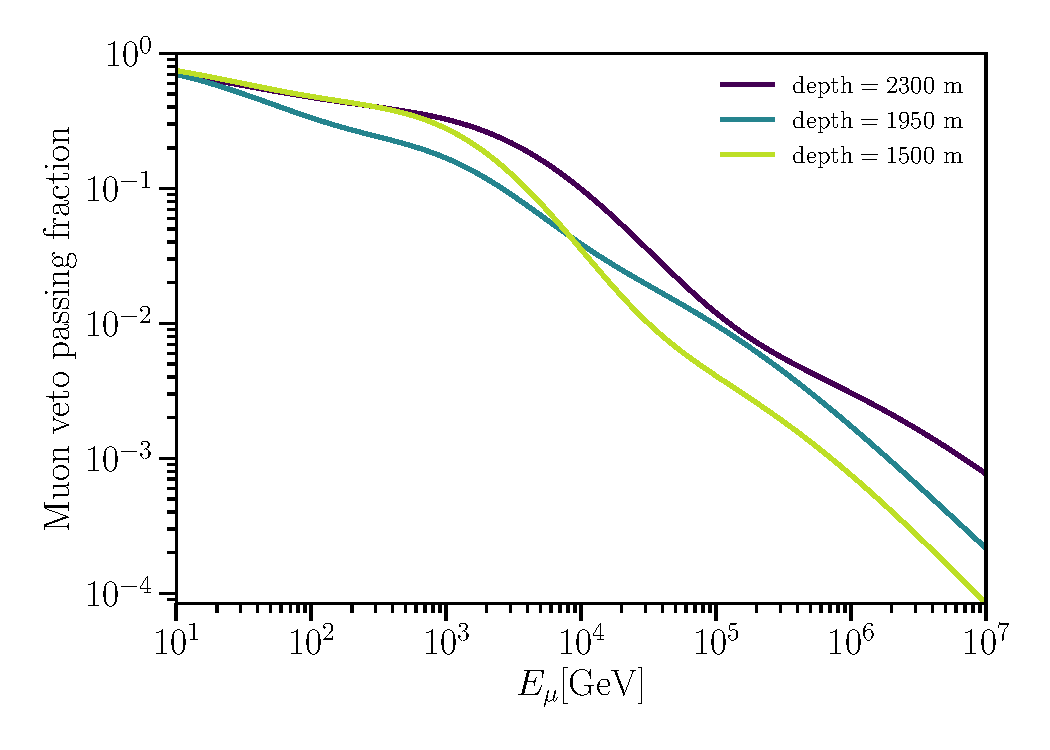
\includegraphics[width=\linewidth]{figures/hese_paper/plight}
	\internallinenumbers
	\caption{\textbf{\textit{Muon veto passing fraction.}} Each line shows the fraction of muons of a given energy, $E_\mu$, that pass without triggering the veto when entering the detector at a particular depth.
		Three depths are shown: 1500, 1950, and 2300 meters from the surface; with lines of darkening color as the depth increases.
		The veto efficiency increases with the muon energy.
		Differences at various depths are due to the changing ice properties and acceptance as a function of depth.}\label{fig:P_light}
\end{figure}

Using the passing fractions in \reffig{fig:P_light} as input and the \nuveto{} code provided in~\cite{Arguelles:2018awr} we calculate the atmospheric passing fraction for each component and flavor using the Hillas-Gaisser H3a~\cite{Gaisser:2013bla,Gaisser:2011cc,Hillas:2006ms} model for the incident cosmic-ray spectra and SIBYLL2.3c~\cite{Riehn:2017mfm} for the hadronic interactions in the air shower.
Using passing fractions derived from alternative cosmic-ray and hadronic interaction models has sub-leading effects in the determination of the astrophysical flux~\cite{Arguelles:2018awr}.
In this work, this was studied by repeating the analysis for different passing fractions that arise from a given combination of cosmic-ray spectrum and hadronic model for a variety of spectra and models that are available in the literature.
We found that the inclusion of these effects in addition to other discrete ice choices mentioned later increases the uncertainty of the astrophysical measurement by at most $\SI{20}\percent$ of existing errors.
In \reffigs{fig:passingfraction_conventional}{fig:passingfraction_prompt} we show the passing fractions for the conventional and prompt neutrino components.
In these figures the left, center, and right panels correspond to $\cos\theta_z$ values of 0.1, 0.3, and 0.9 respectively; the solid lines correspond to muon neutrinos and the dashed lines to electron neutrinos.
In the progression of the panels from left to right, one can see the passing fractions become smaller as one approaches vertical directions.
Vertical muons have the highest probability of reaching the detector, as the overburden they pass through is the smallest.
Though not shown in this figure, the conventional passing fractions differ from neutrinos to anti-neutrinos, see~\cite{Arguelles:2018awr} for details; in the analysis these differences are accounted for and figures for the anti-neutrino passing fractions can be found in~\cite{HESE:datarelease}.%TODO put these figures in the data release webpage
\reffigs{fig:conventional_distribution}{fig:prompt_distribution} show the distributions of conventional and prompt respectively after this correction is applied.
This reduction in atmospheric background is critical for measuring the astrophysical neutrino flux, as the observed down-going fluxes in IceCube would otherwise be comparable in magnitude and remain similar in their angular distribution.
This is best seen when comparing the atmospheric fluxes before and after the veto to the measured astrophysical flux as shown in \reffig{fig:neutrino_spectrum}.

% Plot of the passing fraction for different heights (one line per height) (one panel for each costh [3 values])
\begin{figure*}
	\centering
	\subfloat{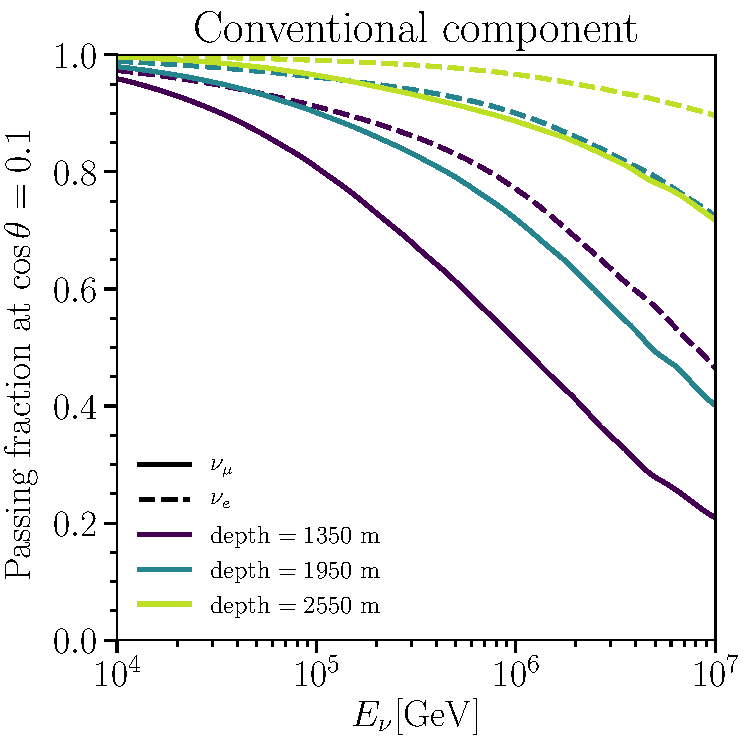
\includegraphics[width=0.3\linewidth]{figures/hese_paper/conv_0_1_passing_fraction}}
	\subfloat{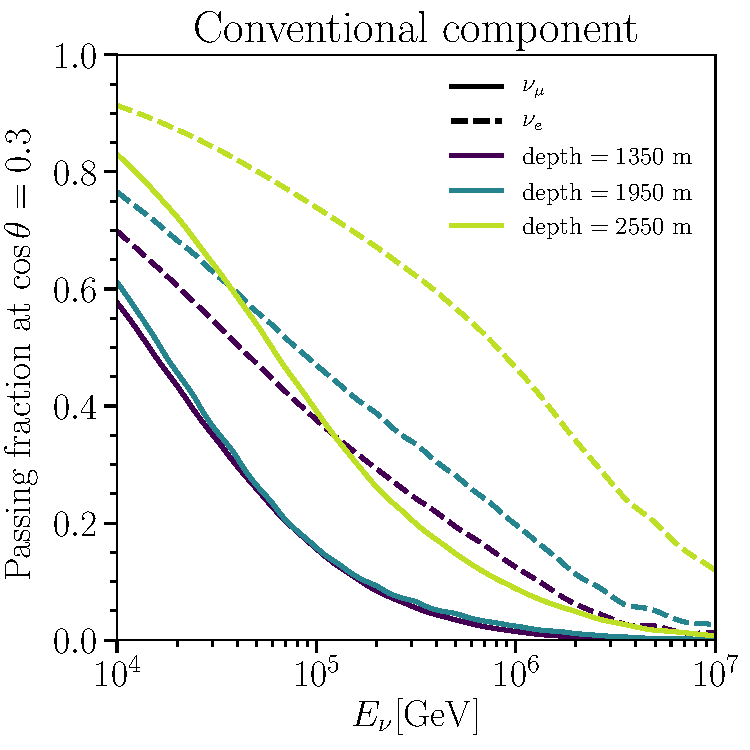
\includegraphics[width=0.3\linewidth]{figures/hese_paper/conv_0_3_passing_fraction}}
	\subfloat{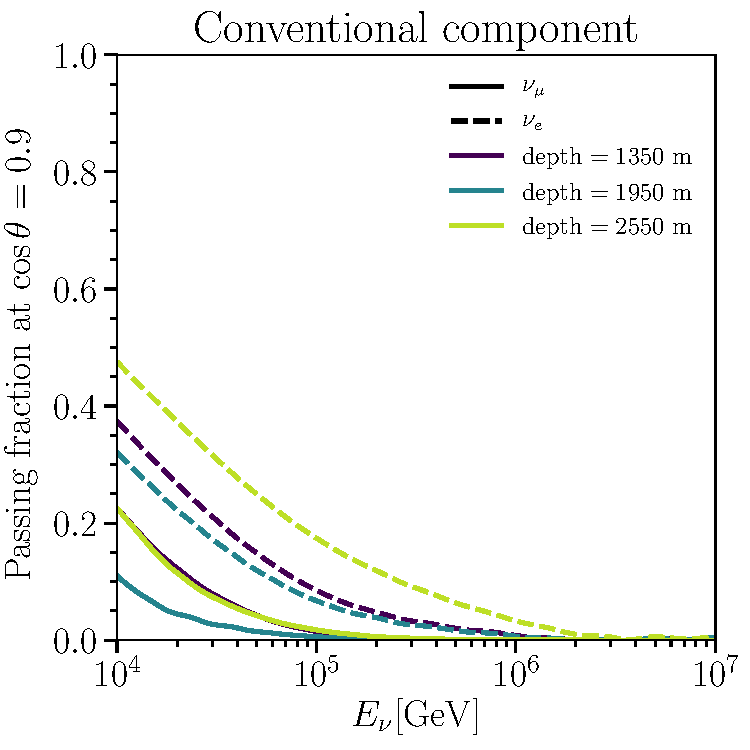
\includegraphics[width=0.3\linewidth]{figures/hese_paper/conv_0_9_passing_fraction}}
	\internallinenumbers
	\caption{\textbf{\textit{Conventional atmopheric component passing fraction.}}
		The atmospheric neutrino passing fraction is shown as a function of the neutrino energy, assuming the Hillas-Gaisser H3a~\cite{Gaisser:2013bla,Gaisser:2011cc,Hillas:2006ms} cosmic-ray model and SIBYLL 2.3c~\cite{Riehn:2017mfm} hadronic interaction model.
		Solid lines correspond to electron neutrinos and dashed lines to muon neutrinos.
		The different colors, from darkest to lightest, are for three different detector depths: 1350, 1950, and 2550 meters below the surface.
		The left, center, and right panel correspond to cosine of the zenith angles 0.1, 0.3, and 0.9 respectively (or zenith angles of $\SI{57}\degree$, $\SI{54.7}\degree$, and $\SI{35.6}\degree$).}\label{fig:passingfraction_conventional}
\end{figure*}

\begin{figure*}
	\centering
	\subfloat{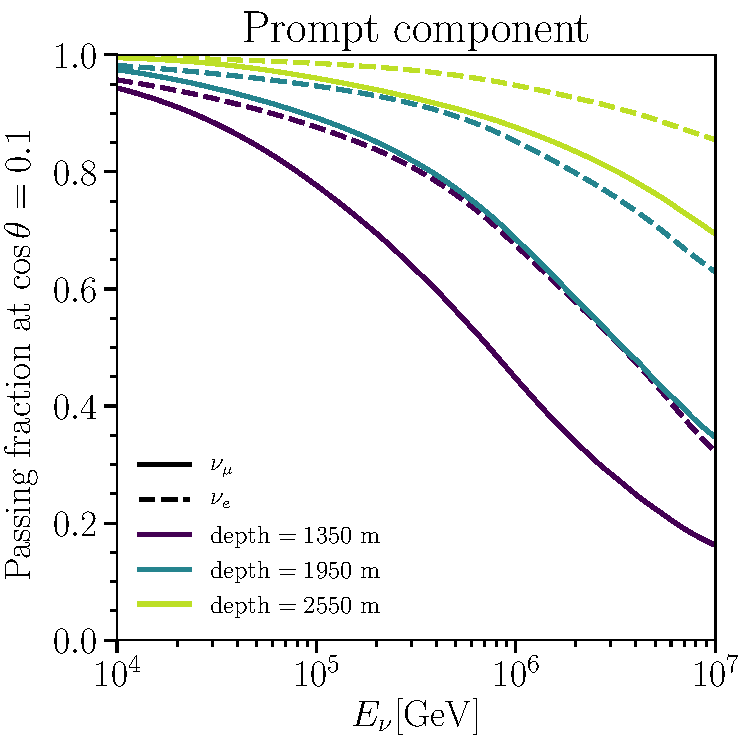
\includegraphics[width=0.3\linewidth]{figures/hese_paper/prompt_0_1_passing_fraction}}
	\subfloat{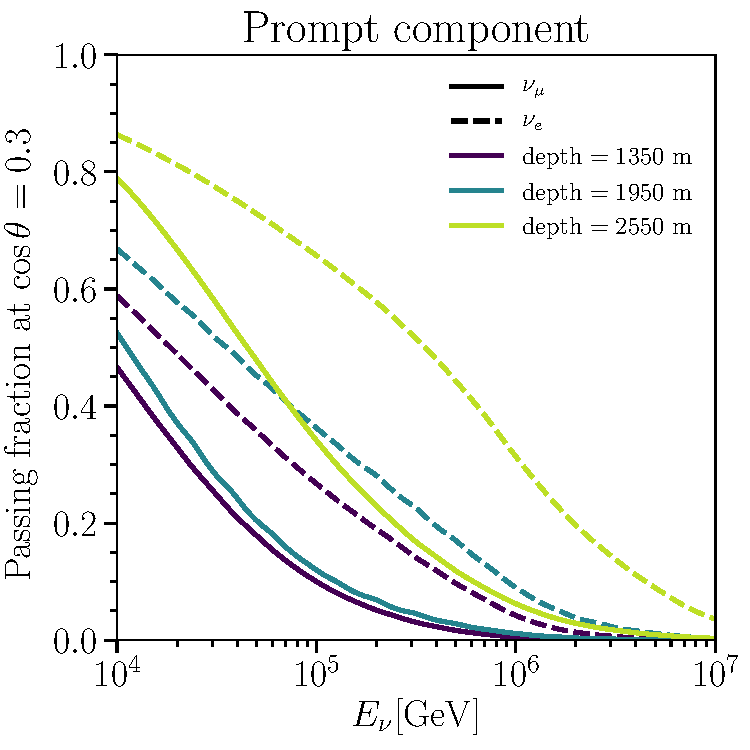
\includegraphics[width=0.3\linewidth]{figures/hese_paper/prompt_0_3_passing_fraction}}
	\subfloat{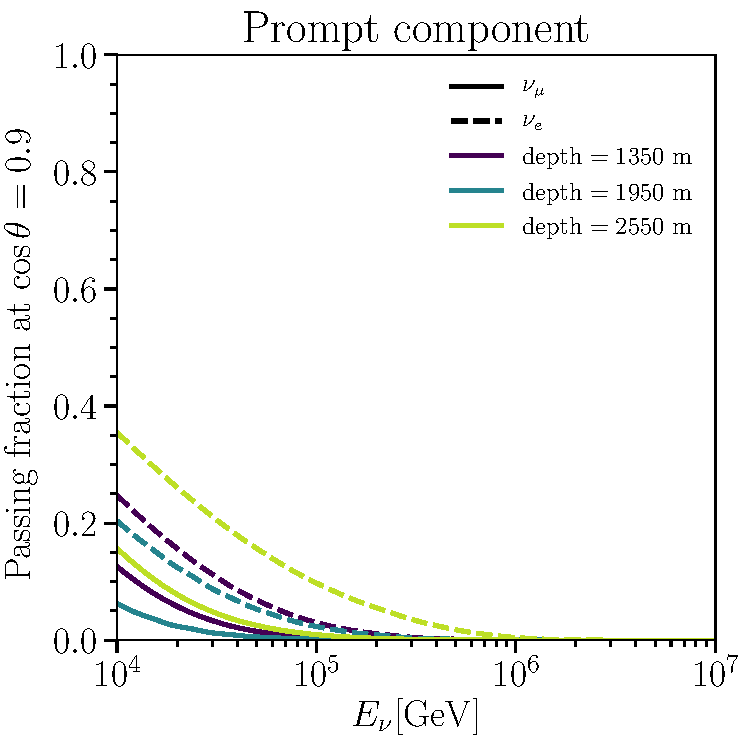
\includegraphics[width=0.3\linewidth]{figures/hese_paper/prompt_0_9_passing_fraction}}
	\internallinenumbers
	\caption{\textbf{\textit{Prompt atmospheric component passing fraction.}} Assumptions and line color coding are the same as in \reffig{fig:passingfraction_conventional}.}\label{fig:passingfraction_prompt}
\end{figure*}

\begin{figure}
	\centering
	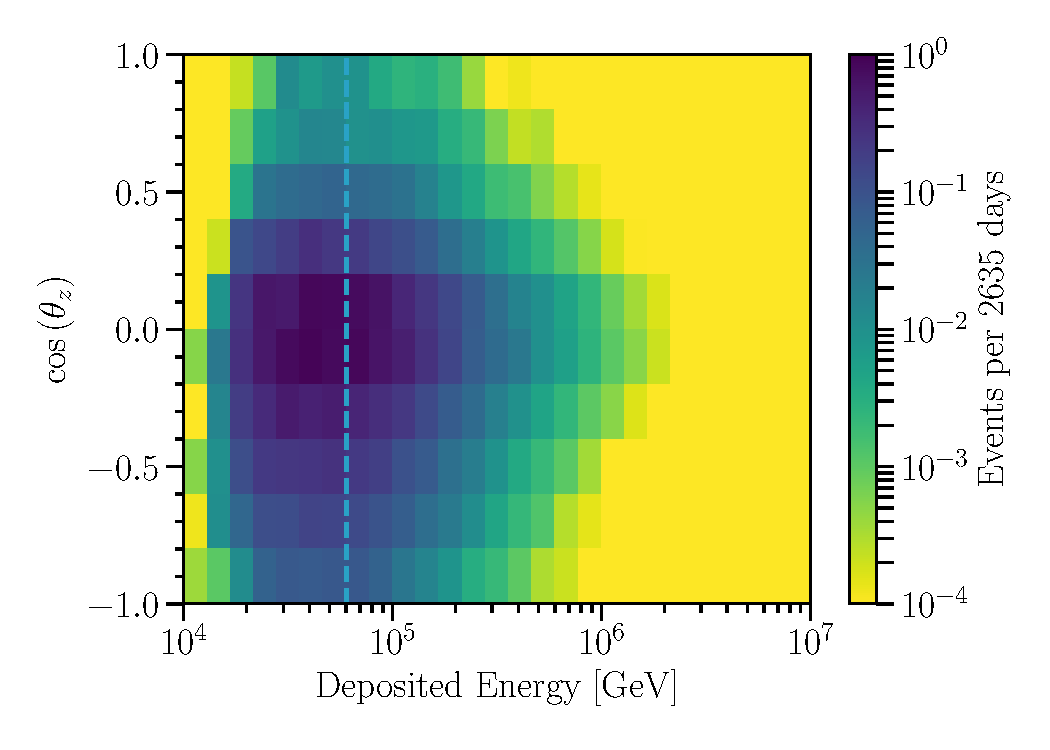
\includegraphics[width=\linewidth]{figures/hese_paper/diffuse_hist_all_conv}
	\internallinenumbers
	\caption{\textbf{\textit{Expected distribution of atmospheric neutrinos produced by pions and kaons in the sample.}} Distribution of neutrinos that pass the veto as a function of the deposited energy and the cosine of the zenith angle assuming nominal values for the nuisance parameters.
		The dashed line at $\SI{60}\TeV$ marks the low energy cut of the analysis.
		See \refsec{sec:systematics} for a discussion of the uncertainties associated with this component.}\label{fig:conventional_distribution}
\end{figure}

\begin{figure}
	\centering
	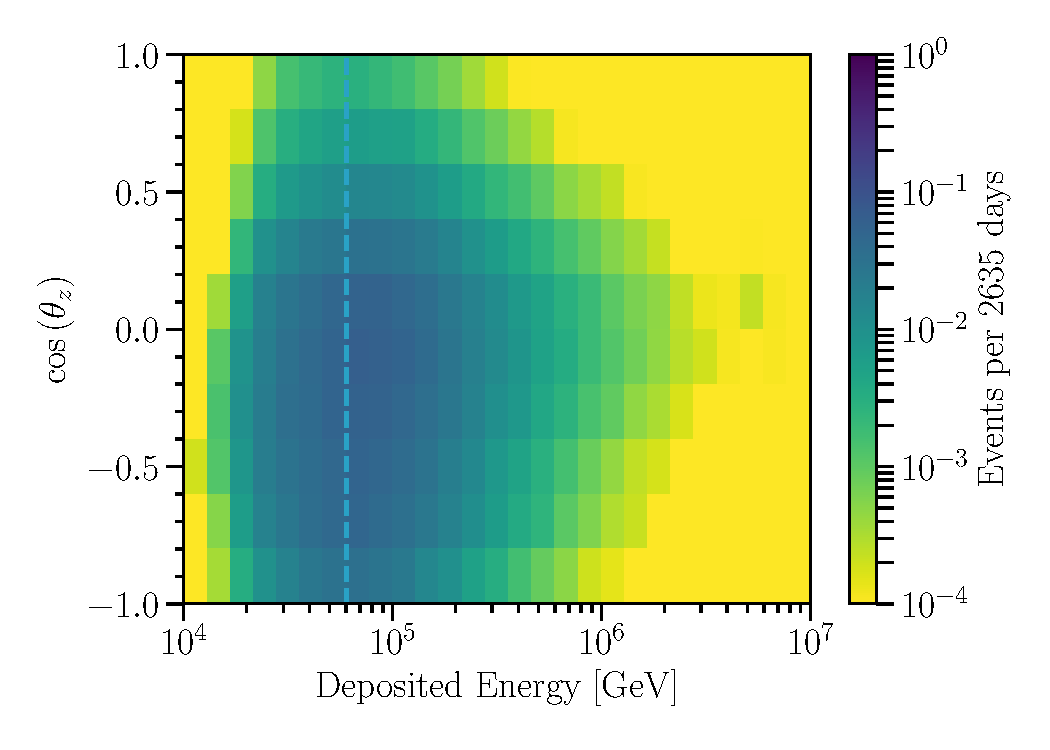
\includegraphics[width=\linewidth]{figures/hese_paper/diffuse_hist_all_prompt}
	\internallinenumbers
	\caption{\textbf{\textit{Expected distribution of atmospheric neutrinos produced by charm hadrons in the sample.}} Distribution of neutrinos that pass the veto as a function of the deposited energy and the cosine of the zenith angle assuming nominal nuisance parameters and production by charmed hadrons.
		The dashed line at $\SI{60}\TeV$ marks the low energy cut of the analysis.
		See \refsec{sec:systematics} for a discussion of the uncertainties associated with this component.}\label{fig:prompt_distribution}
\end{figure}

\begin{figure}
	\centering
	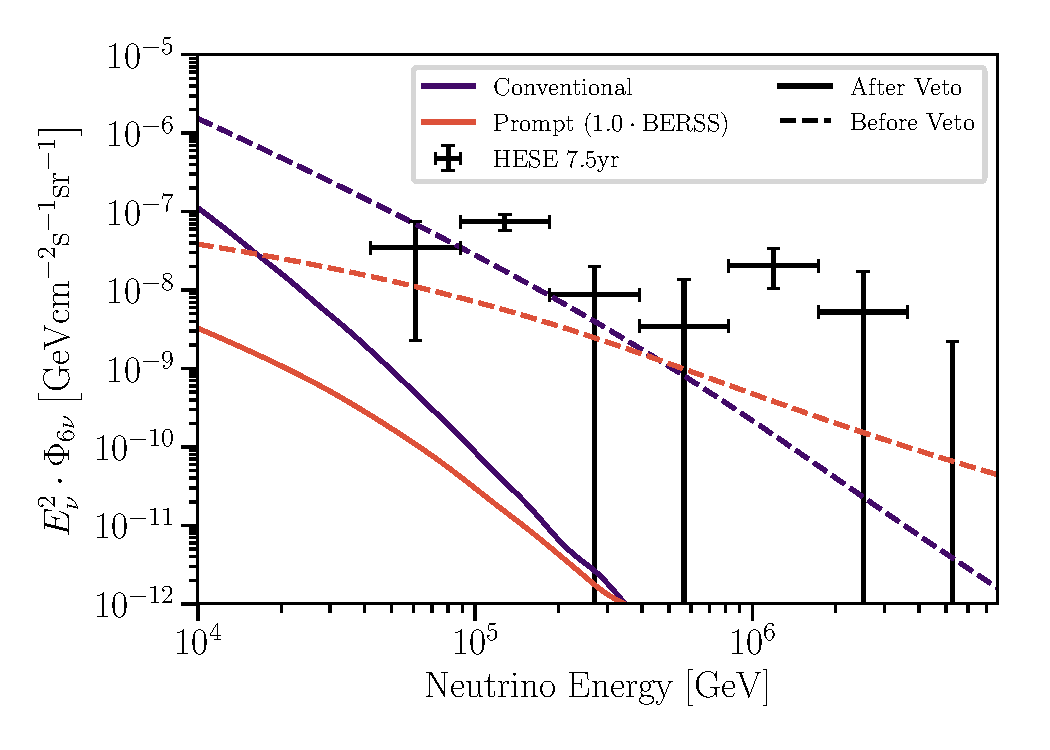
\includegraphics[width=\linewidth]{figures/hese_paper/neutrino_spectrum}
	\internallinenumbers
	\caption{\textbf{\textit{Astrophysical and atmospheric neutrino flux before and after the veto.}} The atmospheric neutrino fluxes considered in this analysis are shown as dashed lines.
		The solid lines show the product of the atmospheric flux with the passing fraction averaged over depth at a zenith angle of $\SI{0}\degree$.
		The frequentist segmented power-law fit of the astrophysical flux as described in \refsec{sec:generic_models} is shown in black.
		See \refsec{sec:systematics} for a discussion of the uncertainties associated with this component.}
	\label{fig:neutrino_spectrum}
\end{figure}

Finally there is also the possibility of single muons that trigger the event selection without a neutrino interaction in the detector and still pass the veto.
The flux of atmospheric muons from cosmic-ray air showers is modelled by a parameterization of muons from air showers simulated with the \CORSIKA~\cite{Heck:1998vt} package assuming the Hillas-Gaisser H4a~\cite{Gaisser:2013bla} cosmic-ray flux model and SIBYLL 2.1~\cite{Ahn:2009wx} hadronic model.
A dedicated single muon simulation, called \MUONGUN~\cite{jvsthesis}, is weighted to this flux. 
Due to the uncertainties in the muon yield of cosmic-ray air showers we use a data-based prior to constrain its normalization and only use the shape from simulation.
A second veto layer inside the original outer veto layer is introduced, and events that trigger the outer veto layer, but do not trigger this second inner veto layer, are tagged as muons that pass the inner veto.
The muon normalization from simulation is re-scaled from $N_\MUONGUN$ to $2.1\cdot N^\mu_\textmd{tagged}$ to match the number of tagged muons while accounting for the relative size of the fiducial volumes.
Thus, the baseline expected muon flux is given by
\begin{linenomath*}
	\begin{align}
	\frac{d^3\Phi}{d E_\mu d \theta_{z,\mu} d d_\mu} ={}& \Phi_\texttt{GaisserH4a}(E_\mu, \theta_{z,\mu},d_\mu)\\* & \cdot \frac{2.1 \cdot N^\mu_\textmd{tagged}}{N_\MUONGUN}
	\end{align}
	\label{eq:muon_scaling}
\end{linenomath*}
where $\Phi_\texttt{GaisserH4a}$ is the aforementioned parameterization; and $E_\mu$, $\theta_{z,\mu}$, and $d_\mu$ are the muon energy, zenith, and depth at injection respectively.
In \reftab{tbl:tag_muons} we list the number of tagged muons observed per year; in total 17 muons were observed.
The expected distribution of passing atmospheric muon events is shown in \reffig{fig:muons} as a function of the deposited energy and reconstructed cosine of the zenith angle.

\begin{figure}
	\centering
	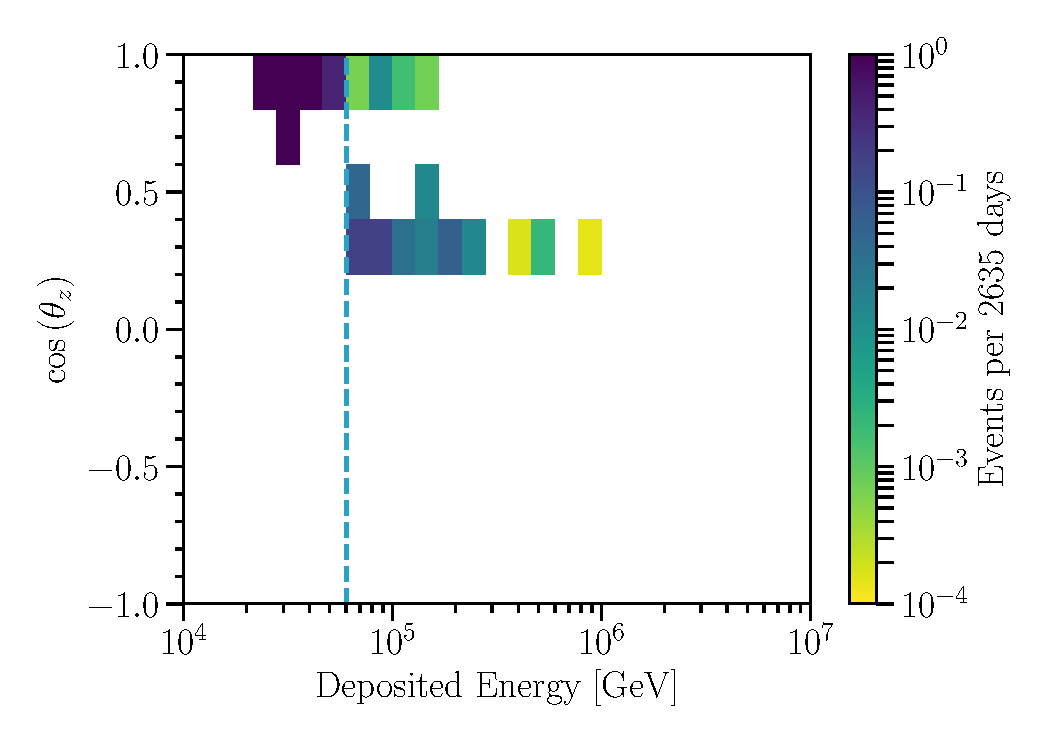
\includegraphics[width=\linewidth]{figures/hese_paper/diffuse_hist_all_muons}
	\internallinenumbers
	\caption{\textbf{\textit{Expected distribution of atmospheric muons in the sample.}} Distribution of muons that pass the veto as calculated with \MUONGUN~as a function of the deposited energy and the cosine of the zenith angle.
		The normalization is set to match the data driven sub-detector study.
		The dashed line at $\SI{60}\TeV$ marks the low energy cut of the analysis.}\label{fig:muons}
\end{figure}

\begin{table}
	\centering
	% year & number of tagged muons
	\begin{tabular}{l r}
		\toprule
		Year & $N^\mu_{tagged}$ \\
		\midrule
		2010 & 2 \\
		2011 & 1 \\
		2012 & 1 \\
		2013 & 1 \\
		2014 & 2 \\
		2015 & 6 \\
		2016 & 2 \\
		2017 & 2 \\
		\midrule
		Total & 17 \\
		\bottomrule
	\end{tabular}
	\internallinenumbers
	\caption{\textbf{\textit{Number of tagged muons per season.}}
		Table shows the number of tagged muons used to construct the muon normalization prior.
		The first year, 2010, used a partial IceCube configuration with 79 strings, the rest of the years of data taking were with the full configuration of 86 strings.}\label{tbl:tag_muons}
\end{table}

\section{Cosmic rays}

\section{Neutrino production in air-showers}

\section{Accounting for veto effects}

\section{Muon backgrounds}
